\documentclass[notes,11pt, aspectratio=169]{beamer}

\usepackage{pgfpages}
% These slides also contain speaker notes. You can print just the slides,
% just the notes, or both, depending on the setting below. Comment out the want
% you want.
\setbeameroption{hide notes} % Only slide
%\setbeameroption{show only notes} % Only notes
%\setbeameroption{show notes on second screen=right} % Both

\usepackage{helvet}
\usepackage[default]{lato}
\usepackage{array}


\usepackage{tikz}
\usepackage{verbatim}
\setbeamertemplate{note page}{\pagecolor{yellow!5}\insertnote}
\usetikzlibrary{positioning}
\usetikzlibrary{snakes}
\usetikzlibrary{calc}
\usetikzlibrary{arrows}
\usetikzlibrary{decorations.markings}
\usetikzlibrary{shapes.misc}
\usetikzlibrary{matrix,shapes,arrows,fit,tikzmark}
\usepackage{amsmath}
\usepackage{mathpazo}
\usepackage{hyperref}
\usepackage{lipsum}
\usepackage{multimedia}
\usepackage{graphicx}
\usepackage{multirow}
\usepackage{graphicx}
\usepackage{dcolumn}
\usepackage{booktabs,tabularx}
\usepackage{bbm}
\usepackage{hyperref}
\newcolumntype{d}[0]{D{.}{.}{5}}

\usepackage{changepage}
\usepackage{appendixnumberbeamer}
\newcommand{\beginbackup}{
   \newcounter{framenumbervorappendix}
   \setcounter{framenumbervorappendix}{\value{framenumber}}
   \setbeamertemplate{footline}
   {
     \leavevmode%
     \hline
     box{%
       \begin{beamercolorbox}[wd=\paperwidth,ht=2.25ex,dp=1ex,right]{footlinecolor}%
%         \insertframenumber  \hspace*{2ex} 
       \end{beamercolorbox}}%
     \vskip0pt%
   }
 }
\newcommand{\backupend}{
   \addtocounter{framenumbervorappendix}{-\value{framenumber}}
   \addtocounter{framenumber}{\value{framenumbervorappendix}} 
}


\usepackage{graphicx}
\usepackage[space]{grffile}
\usepackage{booktabs, fontawesome}

% These are my colors -- there are many like them, but these ones are mine.
\definecolor{blue}{RGB}{0,114,178}
\definecolor{red}{RGB}{213,94,0}
\definecolor{yellow}{RGB}{240,228,66}
\definecolor{green}{RGB}{0,158,115}

\hypersetup{
  colorlinks=false,
  linkbordercolor = {white},
  linkcolor = {blue}
}


%% I use a beige off white for my background
\definecolor{MyBackground}{RGB}{255,253,218}

%% Uncomment this if you want to change the background color to something else
%\setbeamercolor{background canvas}{bg=MyBackground}

%% Change the bg color to adjust your transition slide background color!
\newenvironment{transitionframe}{
  \setbeamercolor{background canvas}{bg=yellow}
  \begin{frame}}{
    \end{frame}
}

\setbeamercolor{frametitle}{fg=blue}
\setbeamercolor{title}{fg=black}
\setbeamertemplate{footline}[frame number]
\setbeamertemplate{navigation symbols}{} 
\setbeamertemplate{itemize items}{-}
\setbeamercolor{itemize item}{fg=blue}
\setbeamercolor{itemize subitem}{fg=blue}
\setbeamercolor{enumerate item}{fg=blue}
\setbeamercolor{enumerate subitem}{fg=blue}
\setbeamercolor{button}{bg=MyBackground,fg=blue,}

% If you like road maps, rather than having clutter at the top, have a roadmap show up at the end of each section 
% (and after your introduction)
% Uncomment this is if you want the roadmap!
% \AtBeginSection[]
% {
%    \begin{frame}
%        \frametitle{Roadmap of Talk}
%        \tableofcontents[currentsection]
%    \end{frame}
% }
\setbeamercolor{section in toc}{fg=blue}
\setbeamercolor{subsection in toc}{fg=red}
\setbeamersize{text margin left=1em,text margin right=1em} 

\newenvironment{wideitemize}{\itemize\addtolength{\itemsep}{10pt}  \setlength\itemsep{.5em}}{\enditemize}

\title[]{How do borrowers find their banks? \\ \vspace{.2cm} The value of individuals in bank relationship formation}
\author[PGP]{Marco Ceccarelli \inst{1}, Christoph Herpfer \inst{2}, Steven Ongena \inst{1}}
\institute[FRBNY]{\small{\begin{tabular}{c c c}
 \inst{1} Swiss Finance Institute and UZH & \hspace*{0.01cm}  & \inst{2} Emory University, Goizueta Business School  \\ \\
        \vspace*{0.5cm}
\includegraphics[scale=0.1]{./figures/sfi_logo}   & \hspace*{0.1cm}  &  
\includegraphics[scale=0.20]{./figures/GBS_hz_280} \vspace{.2cm} \\ 
\multicolumn{3}{c}{SFI Research Days} 
\end{tabular}}}

\date{June 9, 2020}


\begin{document}

%%% TIKZ STUFF
\tikzset{   
        every picture/.style={remember picture,baseline},
        every node/.style={anchor=base,align=center,outer sep=1.5pt},
        every path/.style={thick},
        }
\newcommand\marktopleft[1]{%
    \tikz[overlay,remember picture] 
        \node (marker-#1-a) at (-.3em,.3em) {};%
}
\newcommand\markbottomright[2]{%
    \tikz[overlay,remember picture] 
        \node (marker-#1-b) at (0em,0em) {};%
}
\tikzstyle{every picture}+=[remember picture] 
\tikzstyle{mybox} =[draw=black, very thick, rectangle, inner sep=10pt, inner ysep=20pt]
\tikzstyle{fancytitle} =[draw=black,fill=red, text=white]
%%%% END TIKZ STUFF

% Title Slide
\begin{frame}
  \maketitle
\end{frame}
\note[itemize]{
\item Thanks for being here + coauthors 
\item In this paper we are going to ask a simple question, namely, how do borrowers find their banks? We are going to argue that an important piece of the puzzle is the role played by the individual bankers in facilitating the formation of bank-borrower relationships. 
\item Let me start by providing some anecdotal evidence that bankers do indeed matter and that when they jump ship to a competing bank they take their client portfolio with them. 
}

%%%%%%%%%%%%%%%%%%%%%%%%%%%%%%%%%%%%%%%
% BIG PICTURE QUESTION AND MOTIVATION
%%%%%%%%%%%%%%%%%%%%%%%%%%%%%%%%%%%%%%%
\section{Big picture}
\begin{frame}{Anecdotal evidence}
\centering
  \faQuoteLeft~ [CEO Dan Ariens] approached his lender, LaSalle Bank, to see if it would ramp up his credit line. But LaSalle [\ldots] would never get the additional business. \\ \vspace{.5cm} 
 \onslide<2->{  Ariens, in fact, ended up \textcolor{red}{moving nearly all of his banking relationships to PrivateBancorp.} The Chicago-based bank \textcolor{red}{hired 56 managing directors} in the fourth quarter, \textcolor{red}{most of them from LaSalle}, and posted a 12\% increase in loans compared with the year-ago quarter. \\ \vspace{.5cm} }
 \onslide<3->{  \textbf{\textcolor{red}{ ``It felt natural to stay with the people we knew,'' }} [the CEO] said.~\faQuoteRight \\ \vspace{.5cm} } \hfill  (Chicago Tribune, February 18, 2008) 

   % \faQuoteLeft~ Star bankers are routinely subjected to rough treatment when they jump ship to a rival. [...] Credit Suisse took the war-on-talent to a whole new level when it hired private investigators to tail Iqbal Khan, the bank’s former wealth management chief, \textcolor{red}{fearing he might be poaching talent and stealing business leads} in the days before starting a new job at UBS Group AG, in Zurich.~\faQuoteRight \\ \vspace{.2cm} \hfill  (Fortune, October 1, 2019)
    %The move backfired in spectacular and tragic fashion with the death of a private investigator, the ouster of a top-ranked Credit Suisse official—the CEO’s top lieutenant—and the bank’s reputation in tatters.
 
\end{frame}
\note[itemize]{
\item This example highlights how important personal relationships are in commercial banking }

\begin{frame}{Topics to cover}
  \begin{wideitemize}
    \item Motivation and preview of findings 
    \item Data
    \item Empirical findings:
    \begin{wideitemize} 
      \item Which bankers change employers?
      \item Banks profit when new bankers join 
      \item How do labor market friction spill over into capital markets? 
    \end{wideitemize}
  \end{wideitemize}
\end{frame}

%%%%%%%%%%%%%%%%%%%%%%%%%%%%%%%%%%%%%%%
% MOTIVATION AND PREVIEW
%%%%%%%%%%%%%%%%%%%%%%%%%%%%%%%%%%%%%%%
\begin{frame}{Motivation}
\textcolor{red}{Lending relationships:} 
\begin{wideitemize}
  \item have a large impact on borrowers, e.g., impacting both the availability (Ioannidou, Ongena (JF, 2010)) and pricing of credit (Khwaja,  Mian (AER, 2008))
  \item are a channel through which shocks to the banking system are transmitted to the real sector (e.g. Chodorow-Reich (QJE, 2014))
\end{wideitemize} \vspace{.3cm}

\begin{center}
How are these relationships formed? \textcolor{red}{How do banks and borrowers actually match?} \\ \vspace{.3cm}
\end{center}

\textcolor{red}{The role of bankers:} 
\begin{wideitemize}
  \item bankers are the source of soft information about borrower (Berger, Udell (EJ, 2002))
  \item hence, they ought to play a \textcolor{red}{key role in matching borrowers to banks}
  \item and frictions in the labor market for bankers have \textcolor{red}{consequences in capital markets}
\end{wideitemize} \vspace{.2cm}
\end{frame}
\note[itemize]{
\item We use a novel dataset that contains detailed information on the connections that a banker develops during her employment at a bank and information about when a banker changes employer.
\item Will talk about data in more detail later, but let me give you a brief overview of the findings for now.}

%%%%%%%%%%%%%%%%%%%%%%%%%%%%%%%%%%%%%%%
\begin{frame}{Preview of findings}
\begin{enumerate} 

\item Banks seem to recognize the ability of bankers to bring additional business:
\begin{wideitemize}
    \onslide<2->{ 
      \item Bankers that have \textcolor{red}{more clients} are more likely to get poached by competing banks
     }
\end{wideitemize} \vspace{.2cm}

\onslide<3->{ 
\item Bankers succeed in bringing their previous clients with them at the new bank
\begin{wideitemize}
\onslide<4->{ 
  \item After a commercial banker with an established relationship with a borrower switches to another bank, the \textcolor{red}{likelihood of the borrower following the banker to the new employer increases by 14\%} (ca. 3$\times$  uncond. sample average)
  \item These new client relationships have a \textcolor{red}{significant value for the bank}: Deal volume with these clients increases by 35\%}
\end{wideitemize} \vspace{.2cm}
}

\onslide<5->{ 
\item Frictions in the labor market have spillover effects into capital markets 
\onslide<6->{ 
\begin{wideitemize}
  \item Use gender discrimination lawsuits and absence of female directors as a proxies for less female friendly cultures
  \item Banks with such culture \textcolor{red}{lose female bankers and their clients}
\end{wideitemize}}}
\end{enumerate}
\end{frame}

%%%%%%%%%%%%%%%%%%%%%%%%%%%%%%%%%%%%%%%
% LITERATURE OVERVIEW
%%%%%%%%%%%%%%%%%%%%%%%%%%%%%%%%%%%%%%%
\begin{frame}{Literature review I - Role of bankers}
  \textcolor{red}{Bankers play an important role in the lending process}
  \begin{wideitemize}
    \onslide<2->{ 
    \item Bushman, Gao, Martin, Pacelli (2019) find that bankers are important in determining loan characteristics, especially covenant design  
    \item Frattaroli, Herpfer (2020) find that bankers help firms identify partners for strategic alliances 
    \item Gao, Kleiner, Pacelli (RFS, 2020) find that bankers that structure poorly performing loans face disciplining consequences
    \item Herpfer (2018) finds that strong relationships between a borrower and a banker significantly reduce interest rates }
  \end{wideitemize}

\onslide<3->{  \vspace{.2cm} \textcolor{red}{Our contribution:} Look at the \textcolor{red}{role of bankers} in \textcolor{red}{relationship lending}}
\end{frame}
\note[itemize]{
  \item Nascent literature that examines the role of bankers in the lending process
  \item Our contribution is to bring together the relationship lending literature and the more recent studies on the role of individual bankers and ask what the impact of individuals is on the formation of relationships between banks and their clients
}

\begin{frame}{Literature review II - Relationship lending}
\textcolor{red}{Relationship lending plays a key role for both banks and firms}
\begin{wideitemize}
    \onslide<2->{ 
     \item The ability of banks to create information about their borrowers is at the core of banking (e.g., Berger and Udell, JofB 1995; Berger and Udell, EJ 2002; Diamond, REStud 1984; Petersen and Rajan, JF 1994) 
     \item The soft information of these relationships is concentrated in individual bankers (Liberti and Petersen, RCFS 2019; Karolyi, JF 2018)
     \item Banking relationships play a key role also for the firms, influencing loan conditions (Ioannidou and Ongena, JF 2010) and availability (Ongena and Smith, JFE 2001)
     }
\end{wideitemize} 

\onslide<3->{ \vspace{.2cm}
      \textcolor{red}{What drives the formation of relationships between firms and banks?} \\ 
      \begin{wideitemize} \item Schwert, JF 2018; Petersen and Rahan, QJE 1995; JF 2002;... look at the importance of bank characteristics for the formation of borrower relationships \end{wideitemize} }

\end{frame}
\note[itemize]{
  \item Our paper also relates to the much broader literature that looks at the importance of relationship lending. 
  \item Relationship lending generates soft information that can be used instead of collateral or more generally speaking to monitor borrowers
  \item Berger and Udell, JofB 1995 find that borrowers with relationships pay lower interests and are less likely to pledge collateral 
  \item Petersen and Rajan, JF 1994;  empirically examines how ties between a firm and its creditors affect the availability and cost of funds to the firm ``Relationships are valuable and appear to operate more through quantities rather than prices.''
  \item Karoly JF 2018 - Use executive deaths to show that connections between banks and management make lending more likely
}


%%%%%%%%%%%%%%%%%%%%%%%%%%%%%%%%%%%%%%%
% DATA AND METHODOLOGY
%%%%%%%%%%%%%%%%%%%%%%%%%%%%%%%%%%%%%%%
\section{Data \& methodology}
\begin{frame}[label=data_bankers]{Data I - Individual bankers}
  \begin{columns}[c] % align columns
  \begin{column}{.4\textwidth}
  \resizebox{\textwidth}{!}{
    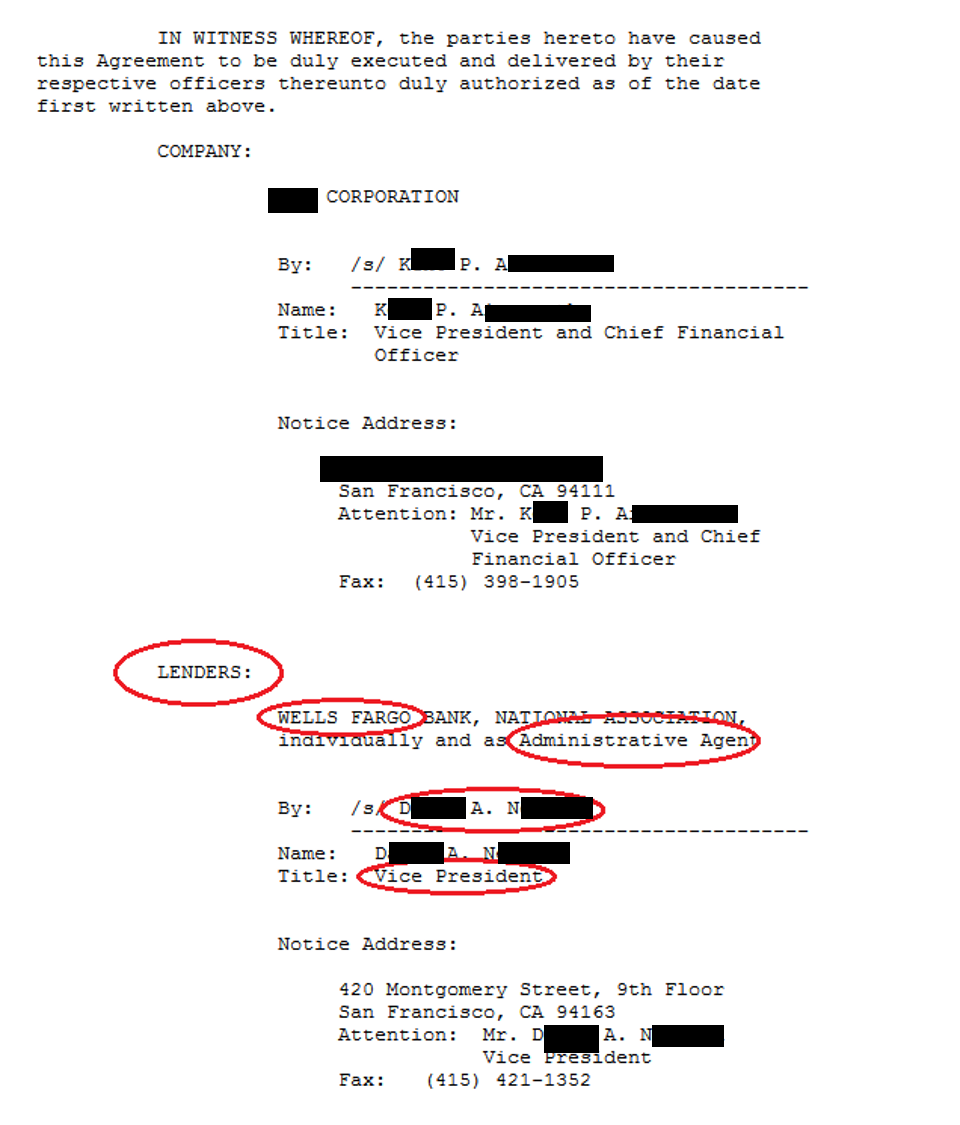
\includegraphics[scale=0.45]{../../Writeup/figures/signature_well_formated.png}
  }
  \end{column}% 
\hfill%
  \begin{column}{.6\textwidth}
    \begin{wideitemize}
      \item Loans considered ``material events''\\ \faArrowRight~ firms must file loan contracts to SEC
      \onslide<2->{
      \item Scrape all 8-K, 10-K, and 10-Q filings and use algorithm developed by Herpfer (2018) to obtain loan information:
      \begin{wideitemize}
          \item \textcolor{red}{Bank Name}
          %\item Bank Role
          \item \textcolor{red}{Person Name}
          %\item Person Title
        \end{wideitemize} }

      \onslide<3->{\item Obtain \textcolor{red}{personal relationships} between banker and clients \textcolor{red}{and} identify \textcolor{red}{bankers that switch} their employer.
      \item From 1996 to 2013, we retrieve some 20,000 bankers that switch 1,066 times.
      \item \hyperlink{appendix_bankers}{\beamergotobutton{Quality-check}} }
    \end{wideitemize}
  \end{column}%
\end{columns}
\end{frame}
\note[itemize]{
\item An 8K can be any sort of announcement of significant corporate information. It's like a press release by the company. A 10K is a formal annual filing that contains the annual financial statements and lots of other information.
}

%%%%% EXAMPLE
\begin{frame}{Data I - Example} \vfill
\begin{figure}[H]  \begin{center}
  \( \begin{array}{cccccc} 
  Yr & Banker & Bank & Firm & Banker~hired & Client~portfolio  \\ \toprule
  2000 & Joe & BofA & GM & 0 & GM \\
  2001 & Joe & BofA & - & 0 & GM \\
  2002 & Joe & BofA & - & 0 & GM  \\
  \marktopleft{a0}2003 & Joe & BofA & HP & 0 & GM;~HP  \\
  2005 & Joe & JPMorgan & GM & 1 & GM;~HP\markbottomright{a0}{red}  \\
  2006 & Joe & JPMorgan & - & 0 & GM;~HP  \\
  \multicolumn{6}{c}{\ldots} \\
  2009 & Joe & JPMorgan & 3M & 0 & GM;~HP;~3M \\ \bottomrule 
  \end{array} \)  \vfill 
\end{center} \end{figure} \vfill
 \only<2>{\centering In 2005 banker Joe switches from BofA to JPMorgan. \\ Crucially, he will bring over his \textcolor{red}{``personal relationships''} to GM and HP.  \vfill \tikz[overlay,remember picture,inner sep=1pt]
\node[draw=red,rounded corners,fit=(marker-a0-a.north west) (marker-a0-b.south east)] {};} 
\end{frame}

%%%%%%%%%%%%%%%%%%%%%%%%%%%%%%%%%%%%%%%%%%%%%%%%%%%%%%%%%%%%%%%%%%%%%%
%%%%%%%%%%%%%%%%%%%%%%%%%%%%%%%%%%%%%%%%%%%%%%%%%%%%%%%%%%%%%%%%%%%%%%
\begin{transitionframe}
  \begin{center}
    \Huge Finding I \\ ~ \\ Which bankers change employers?
  \end{center}
\end{transitionframe}
%%%%%%%%%%%%%%%%%%%%%%%%%%%%%%%%%%%%%%%%%%%%%%%%%%%%%%%%%%%%%%%%%%%%%%
%%%%%%%%%%%%%%%%%%%%%%%%%%%%%%%%%%%%%%%%%%%%%%%%%%%%%%%%%%%%%%%%%%%%%% 

%% SUMMARY STATS IN APPENDIX 
%% ALL OTHER TABLES ALSO IN APPENDIX?

%% SHOW TABLE OF no.clients, no.deals, single/multpl clients

%%%%%%%%%%%%%%%%%%%%%%%%%%%%%%%%%%%%%%%
% MAIN FINDINGS 1 - CLIENT PORTFOLIO
%%%%%%%%%%%%%%%%%%%%%%%%%%%%%%%%%%%%%%%
\section{Main Findings}
\begin{frame}{Finding I - Bankers with a more valuable client portfolio are more likely to switch} 

 \begin{columns}[c] % align columns
  \begin{column}{.55\textwidth}
        \resizebox{\textwidth}{!}{ \centering 
  \begin{tabular*}{\hsize}{@{\hskip\tabcolsep\extracolsep\fill}l*{2}{c}} \toprule 
  Dep. variable:  &\multicolumn{2}{c}{Banker hired (\%)}  \\ \midrule
  \marktopleft{a1} \#Clients-Total\(_{t-1}\)&     0.15***         \\
             &   (3.87)   &\markbottomright{a1}{red} \\
 \marktopleft{a2}  \#Clients-Single contact\(_{t-1}\)& &  0.58*** \\
    & &  (4.14) \\
    \#Clients-Mult. contact\(_{t-1}\)&            &   -0.14** \\
    &&  (-2.10)  \markbottomright{a2}{red} \\
      \midrule Observations    &  39,992   &    39,992  \\
      R-squared       &    0.21   &     0.22 \\
      \midrule Bank-Year FE    & Yes   &      Yes  \\
      \bottomrule
      \end{tabular*} 
  } \end{column}% 
\hfill%
  \begin{column}{.45\textwidth}
     \only<1>{\textcolor{red}{Dependent var.:} Indicator for first year banker appears at new bank \\ \vspace{.2cm}
     \textcolor{red}{Explanatory vars.:} \#Clients that a banker has in her portfolio \\ \vspace{.2cm}  }

     \only<2>{\centering Bankers that have \textcolor{red}{\\relationships to more clients} \\ are more likely to switch \\ \vspace{.2cm} 

     1 std. deviation \#Clients (4.29) increases the chance that this banker switches to a competing bank by 0.65\% \\ (+40\% of the unconditional likelihood)}

     \only<3>{\centering  This is especially true for single-contact clients as they are more likely to follow the banker} 
    
    \only<4>{\centering {\Large Banks seem to recognize the ability of bankers to bring additional business} 
  }
  \end{column}%
\end{columns} 

\only<2>{\tikz[overlay,remember picture,inner sep=1pt] \node[draw=red,rounded corners,fit=(marker-a1-a.north west) (marker-a1-b.south east)] {};}
\only<3>{\tikz[overlay,remember picture,inner sep=1pt] \node[draw=red,rounded corners,fit=(marker-a2-a.north west) (marker-a2-b.south east)] {};}
\end{frame}
\note[itemize]{
  \item  
  }


%%%%%%%%%%%%%%%%%%%%%%%%%%%%%%%%%%%%%%%%%%%%%%%%%%%%%%%%%%%%%%%%%%%%%%
%%%%%%%%%%%%%%%%%%%%%%%%%%%%%%%%%%%%%%%%%%%%%%%%%%%%%%%%%%%%%%%%%%%%%%
\section{Finding II - Initiation and deal volume}
\begin{transitionframe}
  \begin{center}
    \Huge Finding II \\ ~ \\ Does the new bank profit \\ from the switch?
  \end{center}
\end{transitionframe}
%%%%%%%%%%%%%%%%%%%%%%%%%%%%%%%%%%%%%%%%%%%%%%%%%%%%%%%%%%%%%%%%%%%%%%
%%%%%%%%%%%%%%%%%%%%%%%%%%%%%%%%%%%%%%%%%%%%%%%%%%%%%%%%%%%%%%%%%%%%%%

%%%%%%%%%%%%%%%%%%%%%%%%%%%%%%%%%%%%%%%
% EXAMPLE 2 - INITIATION
%%%%%%%%%%%%%%%%%%%%%%%%%%%%%%%%%%%%%%%
\begin{frame}{The perspective of the bank}
\begin{wideitemize}
  \item Explain data structure with bullet points [no time for example probably]
  \item Show Tab 4 (1) to (4) to showcase econometric specification
  \item Tab 5 (4) as full slide 
  \item Tab 7 also as bullet
  \item Mention robustness tests? Probably not, appendix only
\end{wideitemize}
\end{frame}

\note[itemize]{
  \item Introduce 2 new variables, the first initiation takes the value of one the first time that a bank initiates contact with a new firm
  \item Initiation covers both ``organic'' growth and the clients that are brought over by bankers
  \item Relationship acquired, takes the value of 1 for all deals that the new bank makes with the old clients of banker Joe
}

%%%%%%%%%%%%%%%%%%%%%%%%%%%%%%%%%%%%%%%%%%%%%%%%%%%%%%%%%%%%%%%%%%%%%%
%%%%%%%%%%%%%%%%%%%%%%%%%%%%%%%%%%%%%%%%%%%%%%%%%%%%%%%%%%%%%%%%%%%%%%
\section{Finding III - Lawsuits}
\begin{transitionframe}
  \begin{center}
    \Huge Finding III \\ ~ \\ Bankers' labor market frictions and spillovers into capital markets 
  \end{center}
\end{transitionframe}

\begin{frame}{Labor market frictions}
\begin{wideitemize}
  \item Explain setting and how we measure female unfriendly culture
  \item Tab 8 (1)-(3) in slides, (4) as bullet
  \item Tab 9 in slides but quick; Tab 10 as bullet
\end{wideitemize}
\end{frame}

% %%%%%%%%%%%%%%%%%%%%%%%%%%%%%%%%%%%%%%%
% % DATA 2 - INITIATION SUMMARY STATS
% %%%%%%%%%%%%%%%%%%%%%%%%%%%%%%%%%%%%%%%
% \begin{frame}{Data II - Summary statistics}
% \makebox[\linewidth][c] {\centering
%   \begin{tabular}{lcccccc}
%                         &           N&         p25&        mean&         p50&         p75&          sd\\
% \midrule
% \marktopleft{a1}Initiation\_strict (\%)&     972,090&        0.00&        4.74&        0.00&        0.00&       21.25\markbottomright{a1}{red}\\
% \marktopleft{a2}Initiation (\%)     &     972,090&        0.00&        5.19&        0.00&        0.00&       22.19\markbottomright{a2}{red}\\
% \marktopleft{a3}Rel\_acq (\%)       &     972,090&        0.00&        2.93&        0.00&        0.00&       16.86\markbottomright{a3}{red}\\
% \marktopleft{a4}Rel\_acq\(^{5yr}\) (\%)&     958,303&        0.00&        1.53&        0.00&        0.00&       12.28\\
% Rel\_acq\(^{abs}\) (\%)&     946,223&        0.00&        0.27&        0.00&        0.00&        5.23\markbottomright{a4}{red}\\
% \marktopleft{a5}Volume - All deals  &     972,090&        0.00&       75.86&        0.00&        0.00&      806.00\markbottomright{a5}{red}\\
% \marktopleft{a6}Volume - Bonds      &     972,090&        0.00&       25.61&        0.00&        0.00&      376.80\\
% Volume - SEOs       &     972,090&        0.00&        5.15&        0.00&        0.00&      139.88\\
% Volume - Synd. Loans&     972,090&        0.00&       38.25&        0.00&        0.00&      490.65\markbottomright{a6}{red}\\
% \bottomrule \vspace{.2cm}
%   \end{tabular}
% }
% \centering 
% \only<1>{Collapse dataset at the \textcolor{red}{bank $\times$ firm $\times$ year} level \& add bank-firm deals \\ (loans, bonds, and SEOs) w/o banker information \\ \vspace{.1cm}~ \faArrowRight~ Total of 50k loans, 25k bonds, and 13k SEOs} %(some deals counted multiple times if they are closed jointly by more than one bank)
% \only<2>{Initiation\_strict identifies \textcolor{red}{1st time interaction} between a bank and a firm \\~  \\ \vspace{.1cm}~ \tikz[overlay,remember picture,inner sep=1pt] \node[draw=red,rounded corners,fit=(marker-a1-a.north west) (marker-a1-b.south east)] {};}
% \only<3>{Initiation also includes deals with \textcolor{red}{stale clients} (no deal in more than 5yrs) \\~  \\ \vspace{.1cm}~ \tikz[overlay,remember picture,inner sep=1pt] \node[draw=red,rounded corners,fit=(marker-a2-a.north west) (marker-a2-b.south east)] {};}
% \only<4>{Rel\_acq takes the value of 1 for \textcolor{red}{all pairs of new\_bank$\times$old\_client$\times$yr}, \\ for all years after the switch  \\ \vspace{.1cm}~ \tikz[overlay,remember picture,inner sep=1pt] \node[draw=red,rounded corners,fit=(marker-a3-a.north west) (marker-a3-b.south east)] {};}
% \only<5>{Rel\_acq${^{5yr}}$ and Rel\_acq$^{abs}$ take the value of 1, \\ for \textcolor{red}{5-yrs and 1-yr after the switch} and set to missing afterwards  \\ \vspace{.1cm}~ \tikz[overlay,remember picture,inner sep=1pt] \node[draw=red,rounded corners,fit=(marker-a4-a.north west) (marker-a4-b.south east)] {};}
%  \only<6>{Volume - All deals is \textcolor{red}{the sum of all deals} (loans, bonds, SEOs) that \\ a bank closes with a borrower within a year (in USDmm)  \\ \vspace{.1cm}~ \tikz[overlay,remember picture,inner sep=1pt] \node[draw=red,rounded corners,fit=(marker-a5-a.north west) (marker-a5-b.south east)] {};}
%   \only<7>{Volume of deals that a bank closes during a year \textcolor{red}{by deal type} (UDSmm) \\~  \\ \vspace{.1cm}~  \tikz[overlay,remember picture,inner sep=1pt] \node[draw=red,rounded corners,fit=(marker-a6-a.north west) (marker-a6-b.south east)] {};}
% \end{frame}

% \note[itemize]{
% \item The deals don't sum up because the data is at the banker-bank level, i.e., a deal can be counted multiple times at different banks 
% \item The median is 0 all the time because you fill in the gaps and treat years with no deals as explicit zero deals
%   \item Conditional on having a deal, the size of bonds (26k) is 1.5x larger than that of synd loans (50k)
%   \item SEOs are the smallest of the lot (12.8k)
% }

% %%%%%%%%%%%%%%%%%%%%%%%%%%%%%%%%%%%%%%%
% % MAIN FINDINGS 2.1 - INITIATION
% %%%%%%%%%%%%%%%%%%%%%%%%%%%%%%%%%%%%%%%
% \begin{frame}[label=finding2_init]{Finding IIa - Does the new bank profit from the switch?}
%  \begin{columns}[c] % align columns
%   \begin{column}{.65\textwidth}
%     \resizebox{\textwidth}{!}{ \centering 
%       \begin{tabular*}{\hsize}{@{\hskip\tabcolsep\extracolsep\fill}l*{4}{c}}
%  \toprule Dep. variable: &\multicolumn{4}{c}{Initiation}                                  \\\cmidrule(lr){2-5}
%                 &\multicolumn{1}{c}{(1)}   &\multicolumn{1}{c}{(2)}   &\multicolumn{1}{c}{(3)}  &\multicolumn{1}{c}{(4)}  \\
% \midrule
% \marktopleft{a1}Rel\_acq        &     0.07** &     0.09** & 0.13*** &    0.14***   \\
%                 &   (2.37)   &   (2.38)  &      (3.58)  &   (3.80)\markbottomright{a1}{red}   \\
% \midrule
% Observations    &  861,444   &  861,444   &  861,444   &  861,444   \\
% R-squared       &     0.03   &     0.08 &     0.10    &     0.42     \\
% \midrule 
% Year FE &      Yes   &      Yes   & Yes   &        No    \\
% Firm FE         &      Yes   &       No   &    No   &      No     \\
% \marktopleft{a2}Firm-Bank FE    &       No   &      Yes   &      Yes   &      Yes \\
% Bank-Year FE    &       No   &       No   &      Yes  &    Yes \\ 
% Firm-Bank FE    &       No   &      No   &      No  &      Yes\markbottomright{a2}{red}  \\ \bottomrule
% \end{tabular*}%
%   } \end{column}% 
% \hfill%
%   \begin{column}{.3\textwidth} 
%   \only<2>{\centering  Probability of initiating contact with new firm \\ \textcolor{red}{increases after the \\ bank acquires a personal relationship} \\ \vspace{.2cm} This corresponds to \\ 1.5x - 3x the average unconditional probability of initiation \tikz[overlay,remember picture,inner sep=1pt] \node[draw=red,rounded corners,fit=(marker-a1-a.north west) (marker-a1-b.south east)] {}; }
%   \only<3>{\centering Finding holds under \\ \textcolor{red}{tight FE structure}: \\ Bank $\times$ Year (supply), \\ Firm $\times$ Year (demand), and \\ Firm $\times$ Bank FEs (geographic proximity, compatible strategy etc.) \tikz[overlay,remember picture,inner sep=1pt] \node[draw=red,rounded corners,fit=(marker-a2-a.north west) (marker-a2-b.south east)] {};} 
%   \only<4>{\centering Findings remain virtually unchanged when we: \\ \vspace{.1cm} 
%   \begin{wideitemize} 
%     \item use stricter definition of initiation \\ \hyperlink{appendix_initiation}{\beamergotobutton{Table}}  
%     \item use different treatments (5-yrs \& absorptive) \\
%     \hyperlink{appendix_initiation_treat}{\beamergotobutton{Table}}  
%     \item drop first deal that banker signs at new bank \\
%     \hyperlink{appendix_initiation_nofirst}{\beamergotobutton{Table}}  
%     \end{wideitemize} }
%   \only<5>{\Large \centering The bank increases its borrower base by \textcolor{red}{winning over clients known to the banker}}
%       \end{column}%
% \end{columns}
%  \end{frame}

% \note[itemize]{
%  \item hammer down how strict this specification is: fill out sample, treat all relationships acquired as one from the moment the banker switches (explain why this is so conservative), include all relationships that are never brought over. Also, all other new clients that the bank acquires that are not in the bankers' portfolio count against us 
%   \item Result holds when using the various types of relationship acquired 
%   \item Result counts all years starting from the first time the banker appears at the new bank as rel\_acq=1
%   \item Firm-bank-FE accounts for e.g. time-invariant bank-firm-pair characteristics such as geographic proximity, compatible corporate culture and strategy 
%   \item Bank-year-FE account for changes in supply of lending at the bank level
%   \item Firm-year-FE account for changes in demand at the firm 
%   \item Standard errors are 2-way clustered around banks and bankers (adding time as the third dimension also doesn't change anything)
% }

% %%%%%%%%%%%%%%%%%%%%%%%%%%%%%%%%%%%%%%%
% % MAIN FINDINGS 2.2 - DEAL VOLUME
% %%%%%%%%%%%%%%%%%%%%%%%%%%%%%%%%%%%%%%%
% \begin{frame}[label=finding2_vol]{Finding IIb - Does the new bank profit from the switch?}
%  \begin{columns}[c] % align columns
%   \begin{column}{.65\textwidth}
%     \resizebox{\textwidth}{!}{ \centering 
% \begin{tabular*}{\hsize}{@{\hskip\tabcolsep\extracolsep\fill}l*{4}{c}}
% % \def\sym#1{\ifmmode^{#1}\else\(^{#1}\)\fi}
% \toprule
% Dep. variable: &\multicolumn{4}{c}{Log Deal Volume}                             \\\cmidrule(lr){2-5}
% &\multicolumn{1}{c}{(1)}   &\multicolumn{1}{c}{(2)}   &\multicolumn{1}{c}{(3)}   &\multicolumn{1}{c}{(4)} \\
% \midrule
% \marktopleft{a1}Rel\_acq        &     0.65***&     0.72***&     0.61***&     0.30***\\
%                &   (8.62)   &   (4.09)   &   (5.18)  &   (3.80)\markbottomright{a1}{red}  \\
% \midrule
% Observations    &  809,108   &  809,108   &  809,108   &  809,108   \\
% R-squared       &     0.07   &     0.14   &     0.16   &     0.51   \\
% \midrule
% Year FE &      Yes   &      Yes   &      Yes  &      No  \\
% Firm FE         &      Yes   &       No   &       No   &      No \\
% \marktopleft{a2}Firm-Bank FE    &       No   &      Yes   &      Yes   &      Yes \\
% Bank-Year FE    &       No   &       No   &      Yes  &    Yes \\ 
% Firm-Bank FE    &       No   &      No   &      No  &      Yes\markbottomright{a2}{red}\\
% \bottomrule
% \end{tabular*}%
%   } \end{column}% 
% \hfill%
%   \begin{column}{.3\textwidth} 
%   \only<2>{\centering The banks that acquire relationships when bankers switch \textcolor{red}{close more deals} with the new clients \\ \vspace{.2cm} For the median deal \\ (USD 300mm, conditional on closing), this corresponds to an increase of USD 2.1mm \tikz[overlay,remember picture,inner sep=1pt] \node[draw=red,rounded corners,fit=(marker-a1-a.north west) (marker-a1-b.south east)] {};}
%   \only<3>{\centering This holds under a \textcolor{red}{tight FE structure} \tikz[overlay,remember picture,inner sep=1pt] \node[draw=red,rounded corners,fit=(marker-a2-a.north west) (marker-a2-b.south east)] {};}
%    \only<4>{\centering Findings remain virtually unchanged when: \\ \vspace{.1cm} 
%       \begin{wideitemize} 
%     \item using different treatments (5-yrs \& absorptive)  
%      \\ \hyperlink{appendix_vol_treatment}{\beamergotobutton{Table}} 
%     \item looking at first deal and repeated interaction clients separately 
%      \\ \hyperlink{appendix_vol_first}{\beamergotobutton{Table}} 
%    \end{wideitemize}}
%   \only<5>{\Large \centering The bank \textcolor{red}{increases the volume of deals} with acquired clients \\ \vspace{.3cm} 
%   The increase covers \textcolor{red}{both syndicated lending and bonds} 
%      \\ \hfill \hyperlink{appendix_vol_dscan}{\beamergotobutton{Table}} }
%       \end{column}%
% \end{columns}
% \end{frame}

% \note[itemize]{
%   \item Here you drop relationships that don't come over
%   \item Treat all clients with whom you eventually make deals as rel\_acq from the first year after the switch
%   \item Not so much in SEO sample - consistent with investment banking business being separate from lending
%   \item Clearly, having FEs in there makes the comparison with the sample median not 100\% kosher
% }

% %%%%%%%%%%%%%%%%%%%%%%%%%%%%%%%%%%%%%%%
% % CONCLUSION / EXTENSIONS / NEXT STEPS
% %%%%%%%%%%%%%%%%%%%%%%%%%%%%%%%%%%%%%%%
% \section{Conclusion}
% \begin{frame}{Conclusion}
% In sum, bankers appear to be an important piece in explaining the creation of lending relationships. They \textcolor{red}{facilitate the matching} between firms and banks. \\ \vspace{.5cm} 
% \textcolor{red}{Open questions \& next steps:} 
% \begin{wideitemize}
%   \item \textcolor{red}{Identification} - Sources of exogenous variation in the probability of switching, e.g.,  restrictions in labor mobility or drop in bank performance/executive pay 
%   \item Role of \textcolor{red}{bank culture} - Are bankers more likely to leave banks with a ``toxic culture''?
%   \item Role of \textcolor{red}{demographics} - Are female bankers better at forming strong client relationships? Are they more or less likely to switch banks?
% \end{wideitemize}
% \end{frame}

% \begin{transitionframe}
%   \begin{center}
%     \Huge Thank you!
%   \end{center}
% \end{transitionframe}


% %%%%%%%%%%%%%%%%%%%%%%%%%%%%%%%%%%%%%%%%%%%%%%%%%%%%%%%%%%%%%%%%%%%%%%
% %%%%%%%%%%%%%%%%%%%%%%%%%%%%%%%%%%%%%%%%%%%%%%%%%%%%%%%%%%%%%%%%%%%%%%
% \appendix
% \begin{transitionframe}
%   \begin{center}
%     \Huge Appendix
%   \end{center}
% \end{transitionframe}
% %%%%%%%%%%%%%%%%%%%%%%%%%%%%%%%%%%%%%%%%%%%%%%%%%%%%%%%%%%%%%%%%%%%%%%
% %%%%%%%%%%%%%%%%%%%%%%%%%%%%%%%%%%%%%%%%%%%%%%%%%%%%%%%%%%%%%%%%%%%%%%

% \begin{frame}[label=appendix_bankers]{Data I - Individual bankers: Quality assurance}
% Randomly sample 100 contracts to check quality of data:
% \begin{wideitemize}
%   \item 65\% of contracts feature signatures, other contracts are dropped
%   \item 80\% of signatories are extracted successfully
% \end{wideitemize}
% \vspace{.3cm}
% Talk to various bankers in commercial lending
% \begin{wideitemize}
%   \item Authorization of signature only for high ranking bankers
%   \item Bankers that sign are the ones negotiating
%   \item Titles are at the level of junior seniors
%   \item LinkedIn search: Relationship bankers, commercial bankers     
% \end{wideitemize}
% \hfill \hyperlink{data_bankers}{\beamergotobutton{Back}}
% \end{frame}

% %%%%%%%%%%%%%%%%%%%%%%%%%%%%%%%%%%%%%%%%%%%%%%%%%%%%%%%%%%%%%%%%%%%
% \begin{frame}[label=appendix_tenure]{Finding Ia - Tenure}
%    \resizebox{.8\textwidth}{!}{ \centering 
% \begin{tabular*}{\hsize}{@{\hskip\tabcolsep\extracolsep\fill}l*{6}{c}}
% \toprule
%                 &\multicolumn{6}{c}{Pre-Switch Indicator (\%)}                                \\\cmidrule(lr){2-7}
%                 &\multicolumn{1}{c}{(1)}   &\multicolumn{1}{c}{(2)}   &\multicolumn{1}{c}{(3)}   &\multicolumn{1}{c}{(4)}   &\multicolumn{1}{c}{(5)}   &\multicolumn{1}{c}{(6)}   \\
% \midrule
% Tenure of banker (running)&     0.25** &     0.30***&            &            &            &            \\
%                 &   (2.57)   &   (3.07)   &            &            &            &            \\
 
% Max tenure of banker&            &            &     0.50***&     0.55***&            &            \\
%                 &            &            &   (4.90)   &   (5.66)   &            &            \\
 
% Tenure\(^{25\%-50\%}\)&            &            &            &            &     1.33***&     1.29***\\
%                 &            &            &            &            &   (3.39)   &   (3.44)   \\
 
% Tenure\(^{50\%-75\%}\)&            &            &            &            &     2.37***&     2.31***\\
%                 &            &            &            &            &   (4.02)   &   (3.66)   \\
 
% Tenure\(^{75\%-100\%}\)&            &            &            &            &     2.47***&     2.92***\\
%                 &            &            &            &            &   (3.05)   &   (3.54)   \\
% \midrule
% Observations    &   22,642   &   22,642   &    7,871   &    7,871   &   22,642   &   22,642   \\
% R-squared       &     0.23   &     0.31   &     0.26   &     0.38   &     0.23   &     0.31   \\
% \midrule Year FE &      Yes   &       No   &        Yes   &       No   &        Yes   &       No \\
% Bank FE         &      Yes   &       No   &        Yes   &       No   &        Yes   &       No \\
% Bank-Year FE    &      Yes   &       No   &        Yes   &       No   &        Yes   &       No \\
% \bottomrule
% \end{tabular*} }
% \hfill \hyperlink{finding1}{\beamergotobutton{Back}}
% \end{frame}

% %%%%%%%%%%%%%%%%%%%%%%%%%%%%%%%%%%%%%%%%%%%%%%%%%%%%%%%%%%%%%%%%%%%
% \begin{frame}[label=appendix_key]{Finding Ib - Key bankers}
%    \resizebox{.8\textwidth}{!}{ \centering 
% \begin{tabular*}{\hsize}{@{\hskip\tabcolsep\extracolsep\fill}l*{6}{c}}
% \toprule
%                 &\multicolumn{2}{c}{All bankers}&\multicolumn{2}{c}{Non-key}&\multicolumn{2}{c}{Key}  \\\cmidrule(lr){2-3}\cmidrule(lr){4-5}\cmidrule(lr){6-7}
%                 &\multicolumn{1}{c}{(1)}   &\multicolumn{1}{c}{(2)}   &\multicolumn{1}{c}{(3)}   &\multicolumn{1}{c}{(4)}   &\multicolumn{1}{c}{(5)}   &\multicolumn{1}{c}{(6)}   \\
% \midrule
% \%Bank deals by banker&     0.18***&     0.29***&     0.39***&     0.69***&     0.13***&     0.17***\\
%                 &   (8.08)   &   (9.91)   &   (7.25)   &   (9.28)   &   (4.36)   &   (3.62)   \\
% \midrule
% Observations    &   43,233   &   43,233   &   36,730   &   36,427   &    6,300   &    4,954   \\
% R-squared       &     0.24   &     0.30   &     0.18   &     0.22   &     0.57   &     0.71   \\
% \midrule Year FE &      Yes   &       No   &      Yes   &       No   &      Yes   &       No   \\
% Bank FE         &      Yes   &       No   &      Yes   &       No   &      Yes   &       No   \\
% Bank-Year FE    &       No   &      Yes   &       No   &      Yes   &       No   &      Yes   \\
% \bottomrule
% \end{tabular*}}
% \hfill \hyperlink{finding1}{\beamergotobutton{Back}}
% \end{frame}

% %%%%%%%%%%%%%%%%%%%%%%%%%%%%%%%%%%%%%%%%%%%%%%%%%%%%%%%%%%%%%%%%%%%%%%%%%%%
% %%%%%%%%%%%%%%%%%%%%%%%%%%%%%%%%%%%%%%%%%%%%%%%%%%%%%%%%%%%%%%%%%%%%%%%%%%%
% \begin{frame}[label=appendix_initiation]{Finding IIa - 1. Initiation strict}
%    \resizebox{.8\textwidth}{!}{ \centering 
%    \begin{tabular*}{\hsize}{@{\hskip\tabcolsep\extracolsep\fill}l*{6}{c}}
% \toprule
% Dep. variable: &\multicolumn{5}{c}{Initiation\_strict}                          \\\cmidrule(lr){2-6}
% &\multicolumn{1}{c}{(1)}   &\multicolumn{1}{c}{(2)}   &\multicolumn{1}{c}{(3)}   &\multicolumn{1}{c}{(4)}   &\multicolumn{1}{c}{(5)}   \\
% \midrule
% Rel\_acq        &     0.06** &     0.07** &     0.12***&            &            \\
%                 &   (2.42)   &   (2.51)   &   (4.11)   &            &            \\
 
% Rel\_acq\(^{5yr}\)&            &            &            &     0.11***&            \\
%                 &            &            &            &   (3.88)   &            \\
 
% Rel\_acq\(^{abs}\)&            &            &            &            &     0.06***\\
%                 &            &            &            &            &   (3.32)   \\
% \midrule
% Observations    &  861,444   &  861,444   &  861,444   &  847,106   &  834,470   \\
% R-squared       &     0.03   &     0.07   &     0.40   &     0.39   &     0.39   \\
% \midrule Year FE &      Yes   &      Yes   &       No   &       No   &       No   \\
% Firm FE         &      Yes   &       No   &       No   &       No   &       No   \\
% Firm-Bank FE    &       No   &      Yes   &      Yes   &      Yes   &      Yes   \\
% Bank-Year FE    &       No   &       No   &      Yes   &      Yes   &      Yes   \\
% Firm-Year FE    &       No   &       No   &      Yes   &      Yes   &      Yes   \\
% \bottomrule \end{tabular*}
% }
% \hfill \hyperlink{finding2_init}{\beamergotobutton{Back}}
% \end{frame}

% %%%%%%%%%%%%%%%%%%%%%%%%%%%%%%%%%%%%%%%%%%%%%%%%%%%%%%%%%%%%%%%%%%%%%%%%%%%
% \begin{frame}[label=appendix_initiation_nofirst]{Finding IIa - 2. Ignoring first deal}
%    \resizebox{.8\textwidth}{!}{ \centering 
%    \begin{tabular*}{\hsize}{@{\hskip\tabcolsep\extracolsep\fill}l*{6}{c}}
% \toprule
%                 Dep. variable: &\multicolumn{5}{c}{Initiation}                                  \\\cmidrule(lr){2-6}
%                 &\multicolumn{1}{c}{(1)}   &\multicolumn{1}{c}{(2)}   &\multicolumn{1}{c}{(3)}   &\multicolumn{1}{c}{(4)}   &\multicolumn{1}{c}{(5)}   \\
% \midrule
% Rel\_acq\_nofirst&     0.07** &     0.09** &     0.15***&            &            \\
%                 &   (2.35)   &   (2.35)   &   (3.88)   &            &            \\
 
% Rel\_acq\_nofirst\(^{5yr}\)&            &            &            &     0.14***&            \\
%                 &            &            &            &   (3.61)   &            \\
 
% Rel\_acq\_nofirst\(^{abs}\)&            &            &            &            &     0.09***\\
%                 &            &            &            &            &   (3.63)   \\
% \midrule
% Observations    &  858,844   &  858,844   &  858,844   &  844,504   &  834,668   \\
% R-squared       &     0.03   &     0.08   &     0.42   &     0.41   &     0.41   \\
% \midrule Year FE &      Yes   &      Yes   &       No   &       No   &       No   \\
% Firm FE         &      Yes   &       No   &       No   &       No   &       No   \\
% Firm-Bank FE    &       No   &      Yes   &      Yes   &      Yes   &      Yes   \\
% Bank-Year FE    &       No   &       No   &      Yes   &      Yes   &      Yes   \\
% Firm-Year FE    &       No   &       No   &      Yes   &      Yes   &      Yes   \\
% \bottomrule \end{tabular*}
% }
% \hfill \hyperlink{finding2_init}{\beamergotobutton{Back}}
% \end{frame}

% %%%%%%%%%%%%%%%%%%%%%%%%%%%%%%%%%%%%%%%%%%%%%%%%%%%%%%%%%%%%%%%%%%%%%%%%%%%
% \begin{frame}[label=appendix_initiation_treat]{Finding IIa - 3. Different treatments}
%    \resizebox{.8\textwidth}{!}{ \centering 
%    \begin{tabular*}{\hsize}{@{\hskip\tabcolsep\extracolsep\fill}l*{6}{c}}
% \toprule
%                   Dep. variable: &\multicolumn{5}{c}{Initiation}                                  \\\cmidrule(lr){2-6}
%                 &\multicolumn{1}{c}{(1)}   &\multicolumn{1}{c}{(2)}   &\multicolumn{1}{c}{(3)}   &\multicolumn{1}{c}{(4)}   &\multicolumn{1}{c}{(5)}   \\
% \midrule
% Rel\_acq        &     0.07** &     0.09** &     0.14***&            &            \\
%                 &   (2.37)   &   (2.38)   &   (3.80)   &            &            \\
 
% Rel\_acq\(^{5yr}\)&            &            &            &     0.12***&            \\
%                 &            &            &            &   (3.56)   &            \\
 
% Rel\_acq\(^{abs}\)&            &            &            &            &     0.07***\\
%                 &            &            &            &            &   (3.36)   \\
% \midrule
% Observations    &  861,444   &  861,444   &  861,444   &  847,106   &  834,470   \\
% R-squared       &     0.03   &     0.08   &     0.42   &     0.41   &     0.41   \\
% \midrule Year FE &      Yes   &      Yes   &       No   &       No   &       No   \\
% Firm FE         &      Yes   &       No   &       No   &       No   &       No   \\
% Firm-Bank FE    &       No   &      Yes   &      Yes   &      Yes   &      Yes   \\
% Bank-Year FE    &       No   &       No   &      Yes   &      Yes   &      Yes   \\
% Firm-Year FE    &       No   &       No   &      Yes   &      Yes   &      Yes   \\

% \bottomrule \end{tabular*}
% }
% \hfill \hyperlink{finding2_init}{\beamergotobutton{Back}}
% \end{frame}

% %%%%%%%%%%%%%%%%%%%%%%%%%%%%%%%%%%%%%%%%%%%%%%%%%%%%%%%%%%%%%%%%%%%%%%%%%%%
% %%%%%%%%%%%%%%%%%%%%%%%%%%%%%%%%%%%%%%%%%%%%%%%%%%%%%%%%%%%%%%%%%%%%%%%%%%%
% \begin{frame}[label=appendix_vol_treatment]{Finding IIb - 1. Volume - Different treatment}
%    \resizebox{.8\textwidth}{!}{ \centering 
%  \begin{tabular*}{\hsize}{@{\hskip\tabcolsep\extracolsep\fill}l*{6}{c}}
% \toprule
%                 &\multicolumn{6}{c}{Log Deal Volume}                                          \\\cmidrule(lr){2-7}
%                 &\multicolumn{1}{c}{(1)}   &\multicolumn{1}{c}{(2)}   &\multicolumn{1}{c}{(3)}   &\multicolumn{1}{c}{(4)}   &\multicolumn{1}{c}{(5)}   &\multicolumn{1}{c}{(6)}   \\
% \midrule
% Rel\_acq        &     0.65***&     0.72***&     0.61***&     0.30***&            &            \\
%                 &   (8.62)   &   (4.09)   &   (5.18)   &   (3.80)   &            &            \\
 
% Rel\_acq\(^{5yr}\)&            &            &            &            &     0.70***&            \\
%                 &            &            &            &            &   (6.07)   &            \\
 
% Rel\_acq\(^{abs}\)&            &            &            &            &            &     3.47***\\
%                 &            &            &            &            &            &   (6.58)   \\
% \midrule
% Observations    &  809,108   &  809,108   &  809,108   &  809,108   &  807,764   &  806,292   \\
% R-squared       &     0.07   &     0.14   &     0.16   &     0.51   &     0.16   &     0.16   \\
% \midrule Year FE &      Yes   &      Yes   &       Yes   &       Yes   &       Yes  &       Yes   \\
% Firm FE         &      Yes   &       No   &       No   &       No   &       No&       No   \\
% Firm-Bank FE    &       No   &      Yes   &      Yes   &      Yes   &      Yes   &      Yes   \\
% Bank-Year FE    &       No   &       No   &      Yes   &      Yes   &      Yes   &      Yes   \\
% \bottomrule
% \end{tabular*}
% }
% \hfill \hyperlink{finding2_vol}{\beamergotobutton{Back}}
% \end{frame}

% %%%%%%%%%%%%%%%%%%%%%%%%%%%%%%%%%%%%%%%%%%%%%%%%%%%%%%%%%%%%%%%%%%%%%%%%%%%
% \begin{frame}[label=appendix_vol_first]{Finding IIb - Volume 2. First vs. repeat deals}
%    \resizebox{.8\textwidth}{!}{ \centering 
%  \begin{tabular*}{\hsize}{@{\hskip\tabcolsep\extracolsep\fill}l*{6}{c}}
% \toprule
%                   Dep. variable: &\multicolumn{3}{c}{Volume - First deal}&\multicolumn{3}{c}{Volume - Repeat deals}\\\cmidrule(lr){2-4}\cmidrule(lr){5-7}
%                 &\multicolumn{1}{c}{(1)}   &\multicolumn{1}{c}{(2)}   &\multicolumn{1}{c}{(3)}   &\multicolumn{1}{c}{(4)}   &\multicolumn{1}{c}{(5)}   &\multicolumn{1}{c}{(6)}   \\
% \midrule
% Rel\_acq        &     0.81***&            &            &     1.29***&            &            \\
%                 &  (14.71)   &            &            &  (14.02)   &            &            \\
 
% Rel\_acq\(^{5yr}\)&            &     0.96***&            &            &     1.16***&            \\
%                 &            &  (13.83)   &            &            &  (10.65)   &            \\
 
% Rel\_acq\(^{abs}\)&            &            &     4.74***&            &            &     1.65***\\
%                 &            &            &  (11.62)   &            &            &   (6.43)   \\
% \midrule
% Observations    &  930,913   &  929,477   &  927,926   &  930,913   &  929,477   &  927,926   \\
% R-squared       &     0.18   &     0.22   &     0.83   &     0.38   &     0.35   &     0.37   \\
% \midrule Year FE &      Yes   &      Yes   &      Yes   &      Yes   &      Yes   &      Yes   \\
% Firm FE         &       No   &       No   &       No   &       No   &       No   &       No   \\
% Firm-Bank FE    &      Yes   &      Yes   &      Yes   &      Yes   &      Yes   &      Yes   \\
% Bank-Year FE    &      Yes   &      Yes   &      Yes   &      Yes   &      Yes   &      Yes   \\
% \bottomrule
% \end{tabular*}
% }
% \hfill \hyperlink{finding2_vol}{\beamergotobutton{Back}}
% \end{frame}


% %%%%%%%%%%%%%%%%%%%%%%%%%%%%%%%%%%%%%%%%%%%%%%%%%%%%%%%%%%%%%%%%%%%%%%%%%%%
% \begin{frame}[label=appendix_vol_dscan]{Finding IIb - Volume 3. Deal category}
%    \resizebox{.8\textwidth}{!}{ \centering 
%  \begin{tabular*}{\hsize}{@{\hskip\tabcolsep\extracolsep\fill}l*{6}{c}}
% \toprule
%                  Dep. variable: &\multicolumn{5}{c}{Log Deal Volume - Syndicated Loans}          \\\cmidrule(lr){2-6}
%                 &\multicolumn{1}{c}{(1)}   &\multicolumn{1}{c}{(2)}   &\multicolumn{1}{c}{(3)}   &\multicolumn{1}{c}{(4)}   &\multicolumn{1}{c}{(5)}   \\
% \midrule
% Rel\_acq        &     0.33***&     0.18   &     0.20** &            &            \\
%                 &   (4.62)   &   (1.40)   &   (2.04)   &            &            \\
 
% Rel\_acq\(^{5yr}\)&            &            &            &     0.37***&            \\
%                 &            &            &            &   (3.06)   &            \\
 
% Rel\_acq\(^{abs}\)&            &            &            &            &     1.84***\\
%                 &            &            &            &            &   (5.09)   \\
% \midrule
% Observations    &  574,769   &  574,769   &  574,769   &  574,032   &  573,293   \\
% R-squared       &     0.08   &     0.15   &     0.17   &     0.17   &     0.17   \\
% \midrule Year FE &      Yes   &      Yes   &      Yes   &      Yes   &      Yes   \\
% Firm FE         &      Yes   &       No   &       No   &       No   &       No   \\
% Firm-Bank FE    &       No   &      Yes   &      Yes   &      Yes   &      Yes   \\
% Bank-Year FE    &       No   &       No   &      Yes   &      Yes   &      Yes   \\
% \bottomrule
% \end{tabular*}
% }
% \hfill \hyperlink{finding2_vol}{\beamergotobutton{Back}}
% \end{frame}

% \begin{frame}[label=appendix_vol_bond]{Finding IIb - Volume 3. Deal category}
%    \resizebox{.8\textwidth}{!}{ \centering 
%  \begin{tabular*}{\hsize}{@{\hskip\tabcolsep\extracolsep\fill}l*{6}{c}}
% \toprule
%                 Dep. variable: &\multicolumn{5}{c}{Log Deal Volume - Bonds}                     \\\cmidrule(lr){2-6}
%                 &\multicolumn{1}{c}{(1)}   &\multicolumn{1}{c}{(2)}   &\multicolumn{1}{c}{(3)}   &\multicolumn{1}{c}{(4)}   &\multicolumn{1}{c}{(5)}   \\
% \midrule
% Rel\_acq        &     0.45***&     0.51***&     0.43***&            &            \\
%                 &   (5.31)   &   (5.02)   &   (6.66)   &            &            \\
 
% Rel\_acq\(^{5yr}\)&            &            &            &     0.45***&            \\
%                 &            &            &            &   (6.79)   &            \\
 
% Rel\_acq\(^{abs}\)&            &            &            &            &     2.52***\\
%                 &            &            &            &            &   (4.75)   \\
% \midrule
% Observations    &  288,896   &  288,896   &  288,896   &  287,820   &  286,598   \\
% R-squared       &     0.14   &     0.19   &     0.21   &     0.21   &     0.20   \\
% \midrule Year FE &      Yes   &      Yes   &      Yes   &      Yes   &      Yes   \\
% Firm FE         &      Yes   &       No   &       No   &       No   &       No   \\
% Firm-Bank FE    &       No   &      Yes   &      Yes   &      Yes   &      Yes   \\
% Bank-Year FE    &       No   &       No   &      Yes   &      Yes   &      Yes   \\
% \bottomrule
% \end{tabular*}
% }
% \hfill \hyperlink{finding2_vol}{\beamergotobutton{Back}}
% \end{frame}

% \begin{frame}[label=appendix_vol_seo]{Finding IIb - Volume 3. Deal category}
%    \resizebox{.8\textwidth}{!}{ \centering 
%  \begin{tabular*}{\hsize}{@{\hskip\tabcolsep\extracolsep\fill}l*{6}{c}}
% \toprule
%                 Dep. variable: &\multicolumn{5}{c}{Log Deal Volume - SEOs}                      \\\cmidrule(lr){2-6}
%                 &\multicolumn{1}{c}{(1)}   &\multicolumn{1}{c}{(2)}   &\multicolumn{1}{c}{(3)}   &\multicolumn{1}{c}{(4)}   &\multicolumn{1}{c}{(5)}   \\
% \midrule
% Rel\_acq        &     0.12   &     0.09   &     0.02   &            &            \\
%                 &   (0.94)   &   (0.30)   &   (0.06)   &            &            \\
 
% Rel\_acq\(^{5yr}\)&            &            &            &     0.11   &            \\
%                 &            &            &            &   (0.46)   &            \\
 
% Rel\_acq\(^{abs}\)&            &            &            &            &     0.61   \\
%                 &            &            &            &            &   (1.43)   \\
% \midrule
% Observations    &  201,741   &  201,741   &  201,741   &  201,330   &  200,873   \\
% R-squared       &     0.06   &     0.09   &     0.10   &     0.10   &     0.10   \\
% \midrule Year FE &      Yes   &      Yes   &       No   &      Yes   &      Yes   \\
% Firm FE         &      Yes   &       No   &       No   &       No   &       No   \\
% Firm-Bank FE    &       No   &      Yes   &      Yes   &      Yes   &      Yes   \\
% Bank-Year FE    &       No   &       No   &      Yes   &      Yes   &      Yes   \\

% \bottomrule
% \end{tabular*}
% }
% \hfill \hyperlink{finding2_vol}{\beamergotobutton{Back}}
% \end{frame}
% % Findings with different rel\_acq definitions
% % Findings with initiation interaction 

\end{document}
